% !TeX root =../main.tex
% !TeX spellcheck = en_US



% https://tex.stackexchange.com/questions/64252/tikz-midway-label-on-a-bended-line
% https://texample.net/tikz/examples/p2p-topology/

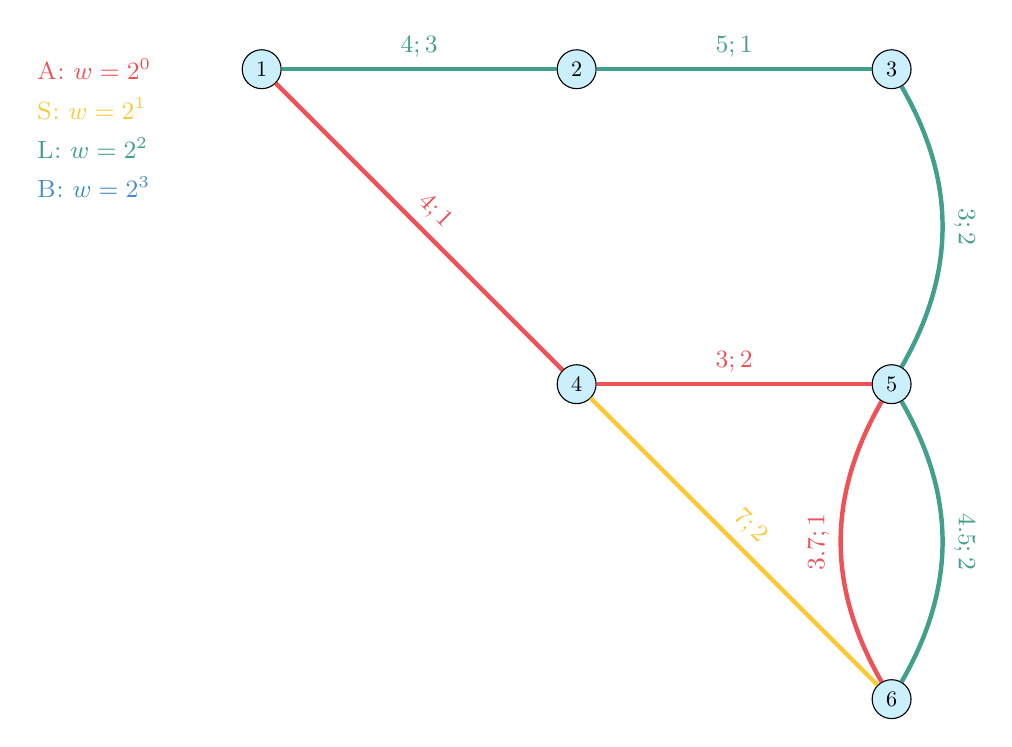
\begin{tikzpicture}[auto, thick]

  % Define Colors
  \definecolor{pinegreen}{cmyk}{0.92,0,0.59,0.25}
  \definecolor{royalblue}{cmyk}{1,0.50,0,0}
  \definecolor{lavander}{cmyk}{0,0.48,0,0}
  \definecolor{violet}{cmyk}{0.79,0.88,0,0}
  \definecolor{red}{cmyk}{0,0.95,0.90,0}
  \definecolor{yellow}{cmyk}{0,0.25,1,0}

  % Node styles
  \tikzstyle{cblue}=[circle, draw, thin,fill=cyan!20, scale=0.8]
  \tikzstyle{qgre}=[rectangle, draw, thin,fill=green!20, scale=0.8]

  \tikzstyle{A_path}=[ultra thick, red, opacity=0.8, font=\small]
  \tikzstyle{S_path}=[ultra thick, yellow, opacity=0.8, font=\small]
  \tikzstyle{B_path}=[ultra thick, royalblue, opacity=0.8, font=\small]
  \tikzstyle{L_path}=[ultra thick, pinegreen, opacity=0.8, font=\small]


  % Nodes
  % \node[cblue] (n_1_1) at (0,0) {1};
  % \node[cblue] (n_2_1) at (4,0) {2};
  \node[cblue] (n_3_1) at (8,0) {6};

  % \node[cblue] (n_1_2) at (0,4) {4};
  \node[cblue] (n_2_2) at (4,4) {4};
  \node[cblue] (n_3_2) at (8,4) {5};

  \node[cblue] (n_1_3) at (0,8) {1};
  \node[cblue] (n_2_3) at (4,8) {2};
  \node[cblue] (n_3_3) at (8,8) {3};



  %  A links
  \draw[A_path] (n_2_2)--  (n_3_2)  node [midway, above, sloped] (TextNode) {$3; 2$};
  \draw[A_path] (n_3_1) to[bend left]   node [midway, above, sloped]  {$3.7; 1$} (n_3_2)  ;
  \draw[A_path] (n_2_2) -- (n_1_3)  node [midway, above, sloped] (TextNode) {$4 ; 1$};

  % S links
  \draw[S_path] (n_2_2) to node [midway, above, sloped] {$7; 2$} (n_3_1);

  %  L lines
  \draw[L_path] (n_1_3) --  (n_2_3)  node [midway, above, sloped] (TextNode) {$4; 3$};
  \draw[L_path] (n_2_3)--  (n_3_3)  node [midway, above, sloped] (TextNode) {$5; 1$};
  % \draw[L_path] (n_3_3) to[out=-20,in=-20]  (n_3_2)  node [midway, above, sloped] (TextNode) {$l=3, b=2$};
  \draw[L_path] (n_3_3) to[bend left] node [midway, above, sloped]   {$3; 2$}    (n_3_2);
  \draw[L_path] (n_3_2) to[bend left]  node [midway, above, sloped] {$4.5; 2$} (n_3_1);

  % B links
  % \draw[B_path] (n_3_1) to node [midway, above, sloped] {$7; 2$} (n_2_1);


  % Legends
  \node[A_path, anchor=west] at (-3,8){\textsc{A:} $w=2^0$};
  \node[S_path,anchor=west] at (-3, 7.5){\textsc{S:} $w=2^1$};
  \node[L_path,anchor=west] at (-3, 7){\textsc{L:} $w=2^2$};
  \node[B_path,anchor=west] at (-3, 6.5){\textsc{B:} $w=2^3$};

\end{tikzpicture}
